\documentclass[12pt,a4paper]{article}
\usepackage[utf8]{inputenc}
\usepackage[portuguese]{babel}
\usepackage{graphicx}

\author{Grupo 157 \and Francisco Sousa 86416 \& João Daniel Silva 86416}
\title{Relatório 1º Projecto de ASA}
\begin{document}
\maketitle

\section{Introdução}
No âmbito da cadeira de Análise e Síntese de Algoritmos foi-nos proposto desenvolver um projeto que consiste em identificar sub-redes regionais numa rede de distribuição
de produtos, considerando as rotas atuais da mesma em que qualquer ponto de distribuição enviar produtos para qualquer outro ponto da rede regional. Isto é, se um ponto \textit{u}
da rede de distribuição tem uma rota para um ponto \textit{v} e do ponto \textit{v} também existe uma rota para o ponto \textit{u}, então ambos os pontos fazem parte da mesma sub-rede regional.

Assim, representamos o problema como um grafo orientado, no qual aplicaremos um algoritmo de procura de componentes fortemente ligadas (SCC), especificamente o \textbf{algoritmo de Tarjan} apresentado na aula teórica.
\section{Descrição da Solução}
Neste grafo, os vértices correspondem a um ponto de distribuição e as arestas às rotas entre os mesmos.

Decidimos fazer a nossa solução em C++, para facilitar a implementação da stack e de algoritmo \textit{sort}, e também para aprofundar o conhecimento nesta linguagem.

\subsection{Estruturas}
Como no projeto não é necessário adicionar ou remover vértices, o grafo foi representado como sendo um \textit{array} de inteiros \textbf{grafD}, em que cada par corresponde a uma aresta.
Para cada vértice cghegámos à conclusão que precisávamos de armazenar 5 propriedades:
\begin{enumerate}
	\item índice da primeira ocorrência como origem de uma aresta no array grafo;
	\item tempo de descoberta para o algoritmo de Tarjan;
	\item menor valor de descoberta atingível por um arco para trás/cruzamento na sub-árvore (low);
	\item informação se está contido na stack; %EXPLICAR PQ
	\item número da SCC em que está contido.
\end{enumerate}
Para armazenar esta informação recorremos a um outro array de inteiros \textbf{tabelaV}, em que cada 5 elementos corresponde às propriedades de um único vértice.

Como no output é esperado que cada ligação entre SCC tenha como origem e destino o mínimo de cada scc, temos outro array que armazena isto \textbf{scc}.

Para facilitar o acesso às variáveis necessárias para a chamada recursiva do Tarjan, recorremos ainda a uma estrutura argumentos \textbf{args\_struct}. Esta contém ponteiros para o grafo, stack, a tabela de vértices, tabela de mínimos de cada scc, além do tempo atual de visita e as dimensões do grafo.
\subsection{Algoritmo}
Começamos por ler do input o tamanho do grafo (número de vértices e arestas), para poder criar as estruturas \textbf{grafD} e \textbf{tabelaV}. De seguida, populamos o primeiro com o resto das ligações lidas.
Procedemos à ordenação das arestas para ter a certeza que as com a mesma origem estavam juntas \textbf{grafO}, facilitando percorrer as adjacências de um vértice, atualizando simultaneamente a \textbf{tabelaV}.
Aplicamos o Tarjan,

\section{Análise}
\subsection{Teórica}
%explicar a stack
\subsection{Experimental}

\begin{figure}[h]
			\centering
			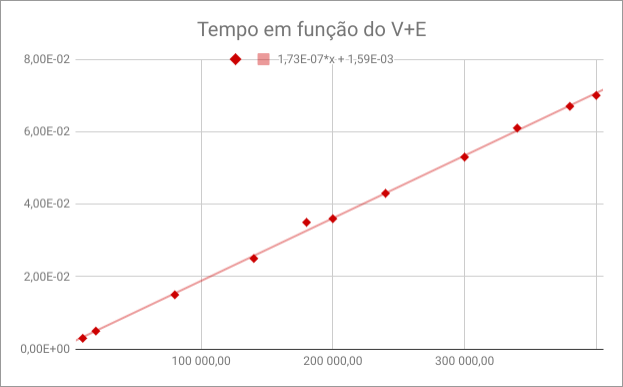
\includegraphics[width=0.5\textwidth]{ss_t(V+E)}
			\caption{Variação do tempo em função do V+E}
\end{figure}
\begin{figure}[h]
			\centering
			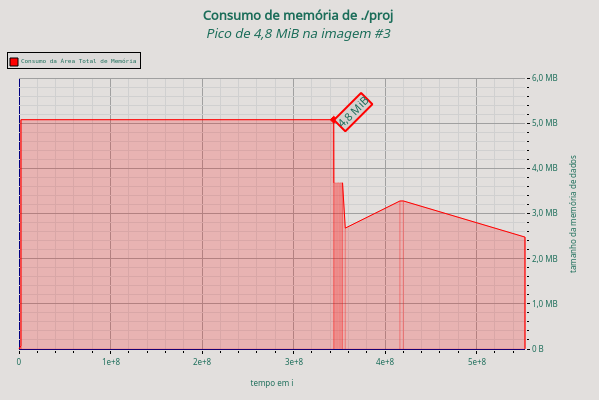
\includegraphics[width=0.5\textwidth]{ss_m(tex)}
			\caption{Variação da memória utilizada em função do tempo de execução}
\end{figure}

\section{Referências}

\end{document}
